\documentclass[a4paper]{article}

%% Language and font encodings
\usepackage[english]{babel}
\usepackage[utf8x]{inputenc}
\usepackage[T1]{fontenc}

%% Sets page size and margins
\usepackage[a4paper,top=3cm,bottom=2cm,left=3cm,right=3cm,marginparwidth=1.75cm]{geometry}

%% Useful packages
\usepackage{amsmath}
\usepackage{float}
\usepackage{graphicx}
\usepackage[colorinlistoftodos]{todonotes}
\usepackage[colorlinks=true, allcolors=blue]{hyperref}
\usepackage{minted}

\usepackage{tikz}
\usetikzlibrary{arrows,positioning,fit,shapes,calc}
\usepackage{algorithm}
\usepackage[noend]{algpseudocode}

\title{Distributed systems}
\author{Oechsel Pierre}


\tikzset{
  treenode/.style = {align=center, inner sep=0pt, text centered, font=\sffamily},
  slave/.style = {treenode, circle, draw, text width=1.5em},
  master/.style = {treenode, circle, draw=red, text width=8em},
}

\begin{document}

\maketitle

\section{First steps}

The main goal of my project was to build a \textbf{decentralized and fault tolerant} network.
Before implementing my current solutions, I thought during a few weeks about other approaches. Even though I didn't implemented them I will write a bit about them.

\subsection{Back to centralisation}

My first thought on which topology to choose was to select the tree topology. Under the condition that the tree is balanced broadcasting, scattering and electing a leader can be done efficiently \cite{tel2000introduction}. We suppose the existence of a master node, which we call \textit{oracle} which maintains a coherent view of the topology. He acts as a server and allows us to maintain the topology of a balanced tree. Adding new node to this tree is not difficult. If one node of the tree fails and become dead, this oracle allows us to rebuild the topology \cite{huang2005performance}. Nodes of the distributed systems are only keeping few informations about the topology: their father and their childs. The root of the tree is linked to the \textit{oracle}.

But the \textit{oracle} can also fail. This event is dramatic: without the oracle we can't maintain a coherent topology anymore. If the root of tree then fails our tree will be splitted in two components without any hopes to restore the situation.
In order to fix this problem, we do not have one \textit{oracle}, but several. They are all linked to each other (here in red). Each oracles are keeping the same copy of the topology.
Now, adding(and updating after a node has failed) a new node to the topology is a bit more tricky. Each node now have two status: either it is an \textit{oracle}, either it is a normal node. So when we are performing operations in order to maintain the topology (like adding a node), a node can switch from being a "basic node" to an "oracle". But under which conditions do we want to execute this switch? This question is tricky as we want to maintain what is stored in the distributed system. The priority should be to always have at least two oracles, but sometimes we might consider it interesting to have more basic nodes.

The previous difficulty and the fact that this idea required to create two different distributed systems (one fully connected for the \textit{oracle} and one in tree topology for the other nodes) prevented me from implementing it.



\begin{figure}[H]
    \centering
    \begin{tikzpicture}[-,level/.style={sibling distance = 8cm/#1,level distance = 1.5cm}, level 1/.style={level distance=2cm}] 
\node [master] {}
    child{node [slave] {}
    child{node [slave] {} 
            child{node [slave] {} 
            	child{node [slave] {} }
							child{node [slave] {}}
            }
            child{node [slave] {}
							child{node [slave] {}}
							child{node [slave] {}}
            }                            
    }
    child{node [slave] {}
            child{node [slave] {} 
            }
            child{node [slave] {}
            }
    }}
; 



\draw (0*360/3: 1cm) node[slave] (sA) {};
\draw (1*360/3: 1cm) node[slave] (sB) {};
\draw (2*360/3: 1cm) node[slave] (sC) {};
 
 \draw[-] (sA) -- (sB);
 \draw[-] (sA) -- (sC);
 \draw[-] (sB) -- (sC);
\end{tikzpicture}
\caption{Three master nodes and  12 basic nodes}
\end{figure}


\subsection{Second idea, ring topology}

Even though the ring topology appear useless because it's not very performant on paper (if we have $n$ nodes and the links are bi-directionnal, we need at least $\frac{n}{2}$ messages for a broadcast for example), its simplicity makes it very interesting for this assignement. So I began to investigate ways to keep this simplicity while allowing it to scale a bit more.
In the end, I had the following idea:
We keep the ring topology. However the nodes of this topology are no more a single agent, but are clusters of $m$ agents.
Inside a cluster all the agents are connected using a fully connected topology. This allow for high performance and also efficiency against failure.

The biggest trick comes from how we are connecting one cluster with the following cluster. We might be tempted by the idea that in each cluster their exists one node that is pointing toward the a node of the next cluster. However, this is a bad idea as we have a point of failure between clusters. We want to avoid this: if a cluster is disconnected from the ring because this node failed we won't be able to reconnect it. My solution was to say the following, given a cluster $X = (x_1, \cdots x_m)$ and $Y = (y_1, \cdots y_m)$ that must be linked in the ring:
\begin{itemize}
    \item Select $\phi: [1, \cdots, m] \mapsto [1, \cdots, m]$ a bijective function.
    \item $x_1$ points toward $y_{\phi(1)}$
    \item $\cdots$
    \item $x_m$ points toward $y_{\phi(m)}$
\end{itemize}

So, even if a node of the cluster $Y$ fails, $X$ is not disconnected as it possess an agent connected to another agent of $Y$.

One other advantage of this approach is that we can adapt existing algorithms for broadcasting, scattering and leader election by combining an algorithm efficient for a ring topology and an algorithm efficient for a fully connected topology.

Unfortunately, as the protocols for adding a new node, or maintaining a topology after a node fails, seemed too long to create and test in the time I had I chose not to go further with this idea.


\begin{figure}[H]
    \centering
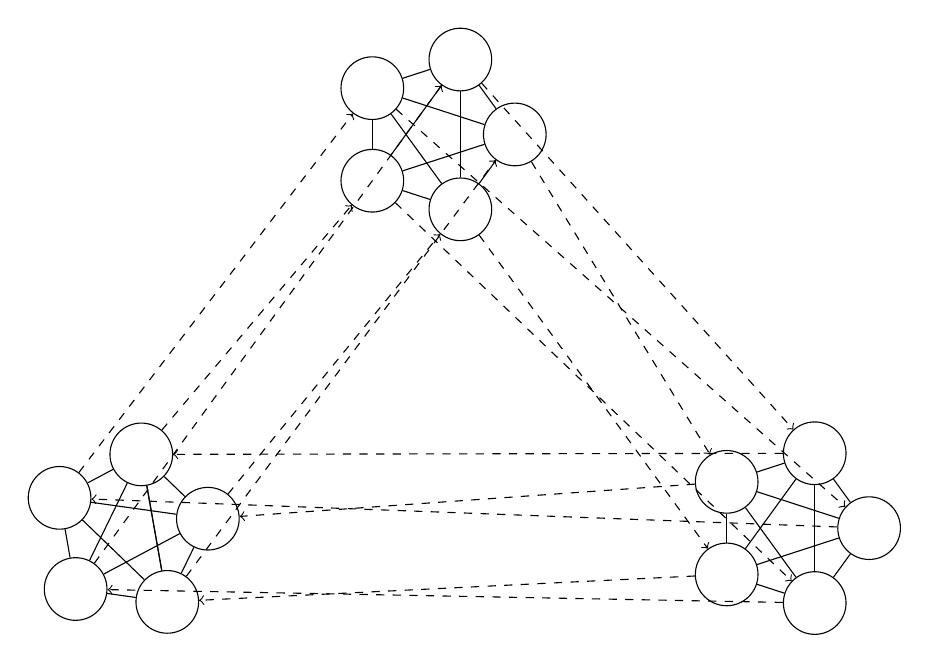
\begin{tikzpicture}[-,level/.style={sibling distance = 5cm/#1,level distance = 1.5cm}] 
\begin{scope}[local bounding box=scope1]
\draw (0*360/5+10: 1cm) node[circle, draw=black, text width=1.5em] (sA) {};
\draw (1*360/5+10: 1cm) node[circle, draw=black, text width=1.5em] (sB) {};
\draw (2*360/5+10: 1cm) node[circle, draw=black, text width=1.5em] (sC) {};
\draw (3*360/5+10: 1cm) node[circle, draw=black, text width=1.5em] (sD) {};
\draw (4*360/5+10: 1cm) node[circle, draw=black, text width=1.5em] (sE) {};
\end{scope}
\begin{scope}[shift={($(scope1.east)+(7cm,0)$)}]
\draw (0*360/5: 1cm) node[circle, draw=black, text width=1.5em] (bA) {};
\draw (1*360/5: 1cm) node[circle, draw=black, text width=1.5em] (bB) {};
\draw (2*360/5: 1cm) node[circle, draw=black, text width=1.5em] (bC) {};
\draw (3*360/5: 1cm) node[circle, draw=black, text width=1.5em] (bD) {};
\draw (4*360/5: 1cm) node[circle, draw=black, text width=1.5em] (bE) {};
\end{scope}
\begin{scope}[shift={($(scope1.east)+(2.5cm,5cm)$)}]
\draw (0*360/5: 1cm) node[circle, draw=black, text width=1.5em] (cA) {};
\draw (1*360/5: 1cm) node[circle, draw=black, text width=1.5em] (cB) {};
\draw (2*360/5: 1cm) node[circle, draw=black, text width=1.5em] (cC) {};
\draw (3*360/5: 1cm) node[circle, draw=black, text width=1.5em] (cD) {};
\draw (4*360/5: 1cm) node[circle, draw=black, text width=1.5em] (cE) {};
\end{scope}
 
\draw[-] (sA) -- (sB);
\draw[-] (sA) -- (sC);
\draw[-] (sA) -- (sD);
\draw[-] (sA) -- (sE);
\draw[-] (sB) -- (sC);
\draw[-] (sB) -- (sD);
\draw[-] (sB) -- (sE);
\draw[-] (sB) -- (sE);
\draw[-] (sC) -- (sD);
\draw[-] (sC) -- (sE);
\draw[-] (sD) -- (sE);



\draw[-] (bA) -- (bB);
\draw[-] (bA) -- (bC);
\draw[-] (bA) -- (bD);
\draw[-] (bA) -- (bE);
\draw[-] (bB) -- (bC);
\draw[-] (bB) -- (bD);
\draw[-] (bB) -- (bE);
\draw[-] (bB) -- (bE);
\draw[-] (bC) -- (bD);
\draw[-] (bC) -- (bE);
\draw[-] (bD) -- (bE);


\draw[-] (cA) -- (cB);
\draw[-] (cA) -- (cC);
\draw[-] (cA) -- (cD);
\draw[-] (cA) -- (cE);
\draw[-] (cB) -- (cC);
\draw[-] (cB) -- (cD);
\draw[-] (cB) -- (cE);
\draw[-] (cB) -- (cE);
\draw[-] (cC) -- (cD);
\draw[-] (cC) -- (cE);
\draw[-] (cD) -- (cE);


\path[->, dashed]
(sC) edge node {} (cC)
(sA) edge node {} (cE)
(sD) edge node {} (cB)
(sE) edge node {} (cA)
(sB) edge node {} (cD)

(bA) edge node {} (sC)
(bB) edge node {} (sB)
(bC) edge node {} (sA)
(bD) edge node {} (sE)
(bE) edge node {} (sD)

(cA) edge node {} (bC)
(cE) edge node {} (bD)
(cC) edge node {} (bA)
(cD) edge node {} (bE)
(cB) edge node {} (bB);

\end{tikzpicture}
\caption{Exemple for a ring of 3 clusters of 5 nodes}
\end{figure}


\section{Welcome Kademlia}

Finally after discussing with other people and doing a bit more of research I chose to implement something approaching Kademlia \cite{maymounkov2002kademlia}. This decision was supported by several reasons:
\begin{itemize}
    \item It allowed me to understand how a "real life" system was working
    \item Its simplicity was intriguing me
\end{itemize}

\section{Choice of implementations}

\subsection{OTP}

As I wanted to learn about erlang during this homework, I chose to follow OTP's guideline. This choice allowed me to have a code a bit cleaner, and mostly to use the full power of Erlang (supervisors, monitors, ...) in a simple way.
However, this decision drasticly decreases my development speed in a first time. As I wasn't a proficient erlang programmer at the start of the project, I spend a lot of time to understand simple things.

OTP also brought a big technical difficulty. Question 4.a asked to be able to spawn an agent remotely given a node name. Without OTP we only need to send the modules used by the agent to the remote node. Here, as I have an OTP application it is not as easy. Therefore, I've proceeded as follow:
\begin{itemize}
    \item Create a new module, \verb|client.erl| which contains everything needed to interact with other agents from the CLI. It is also responsible to start an agent on a remote node
    \item Send \verb|client.erl| to the remote node
    \item Zip the \verb|ebin| folder of the application
    \item Send it on the remote node
    \item Unzip it
    \item Add the destination folder on the remote node to its path
    \item Start the application on the remote note
\end{itemize}

\subsection{Asynchronicity}

Kademlia needs asynchronicity in order to work well. In the original paper, the author advises the use of UDP sockets. Instead, I chose to base myself upon erlang's communications. I still took great care to provide asynchrone method when I can. 
In order to ease my task, I took the following design decisions:
\begin{itemize}
    \item The routing table is executed by a gen\_server launched in another process. As such it is able to maintain a coherent state and to interact with the main process with messages
    \item Algorithms that can take a long time (node lookups, value lookups) are implemented as function executed in another process. For these algorithms I'm making sure to send $\alpha$ messages at the same time (at most).
    \item I'm abusing from call messages and the options to make a call handler return \verb|{noreply, State}|, thus allowing both "asynchronicity" and "synchronicity" at the same time (the caller thinks the call is synchrone, but for the server it is asynchrone).
\end{itemize}


\subsection{Ideas on how to split big files}

When we want to upload a huge file on the network, it is not a good idea to send at once. One big downside of this approach is that when we are refreshing the keys in kademlia, we might have to send the whole file. 
Although I didn't implemented it, I propose the following approach to store huge file on the network:
\subsubsection{Upload}
    et $F$ the file we want to upload and $H$ the sha1 hash function. We suppose we can divide $F$ in chunks $(F_1, \cdots, F_n)$. We define $(k_i)$ as follow:
        \[k_i =\left\{
	\begin{array}{ll}
        H(0 || F_1)  & \text{if } i = 1 \\
        H(1 || k_{i-1} || F_i) & \text{otherwise}
	\end{array}
\right.\]
        We store the $(0||F_1), (1||k_1||F_2), \cdots, (1||k_{n-1}||F_n)$ in the dht and return $k_n$.
        \subsubsection{Download}
        Let $h$ be the hash of the file we want to retrieve. Here is the pseudocode of the algorithm to download the file.

\begin{algorithm}
    \caption{Download of a chunked file}\label{euclid}
\begin{algorithmic}[1]
\Procedure{Download}{h: hash}
\State $m \gets \text{value stored for hash } h$
\If {$\text{first bit of }m\text{is } 0$}
    \State \Return all the bits but the first one
    \Else {}
        \State $h \gets \text{bits 1 to 161 of }m$ 
        \State $x \gets \text{bits 162 to end of }m$
        \State\Return Download($h$) || m
    \EndIf
\EndProcedure
\end{algorithmic}
\end{algorithm}

Thanks to this approach large files are less sensible to failures: as they are divided into different chunks, chunks will be spread along all the nodes.


\bibliographystyle{unsrt}
\bibliography{bib}

\end{document}
